\documentclass[11pt, a4paper]{article}
\usepackage[utf8]{inputenc}
% \usepackage{helvet}
\usepackage{graphicx}

% change default font family from serif to sans-serif
\renewcommand{\familydefault}{\sfdefault}

\title{Projekttitel}
\date{2019-03-05}
\author{John Doe}

\begin{document}
  \pagenumbering{gobble}
  \maketitle
  \newpage

  \tableofcontents
  \newpage


  \pagenumbering{arabic}
  \section{Definitionsphase}
    \subsection{Situationsanalyse}
    \subsection{Auftragsbeschreibung}
    \subsection{Problemdefinition}
    \subsection{Arbeitgeberwuensche (optional)}
    \subsection{Ist-Analyse}
    \subsection{Soll-Konzept}
    \newpage

  \section{Planungsphase}
    \subsection{Kostenplan}
    \subsection{Zeitplan}
    \subsection{Qualitaetssicherungsplan}
    \subsection{Projektstrukturplan}
    \newpage

  \section{Durchfuehrungsphase}
    \subsection{Entwurf}
    \subsection{Design}
    \newpage

  \section{Implementierungsphase}
    \subsection{Tests}
      \subsubsection{Unit Tests}
      \subsubsection{Systemtests}
      \subsubsection{Bedienungstests}
    \subsection{Fachlicher Soll-Ist Vergleich}
    \subsection{Zeitlicher Soll-Ist Vergleich}
    \newpage

  \begin{appendix}
    \listoffigures
    \listoftables
  \end{appendix}
  \newpage

  \section{Figuren}
    \pagenumbering{Roman}
    \subsection{Projektstrukturplan}
      \begin{figure}[h!]
        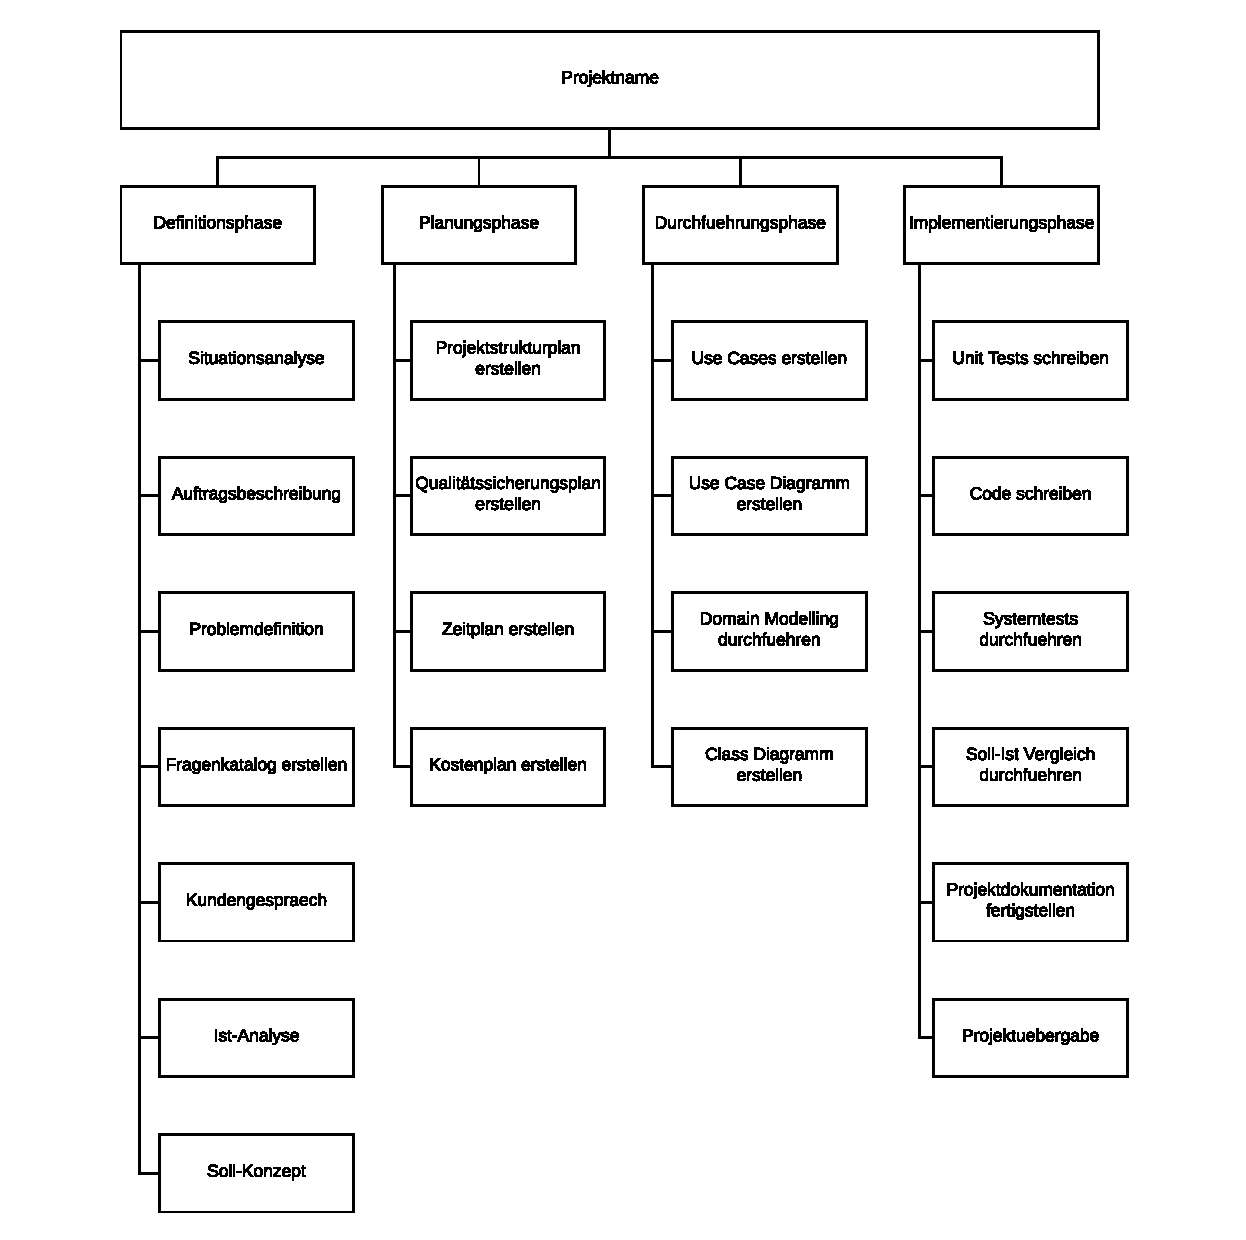
\includegraphics[width=\linewidth]{fig/Projektstrukturplan.pdf}
        \caption{Der Projektstrukturplan}
        \label{fig:psp}
      \end{figure}
      \newpage
    \subsection{Use-Case Diagramm}
    \subsection{Klassendiagramm}
      \begin{figure}[h!]
        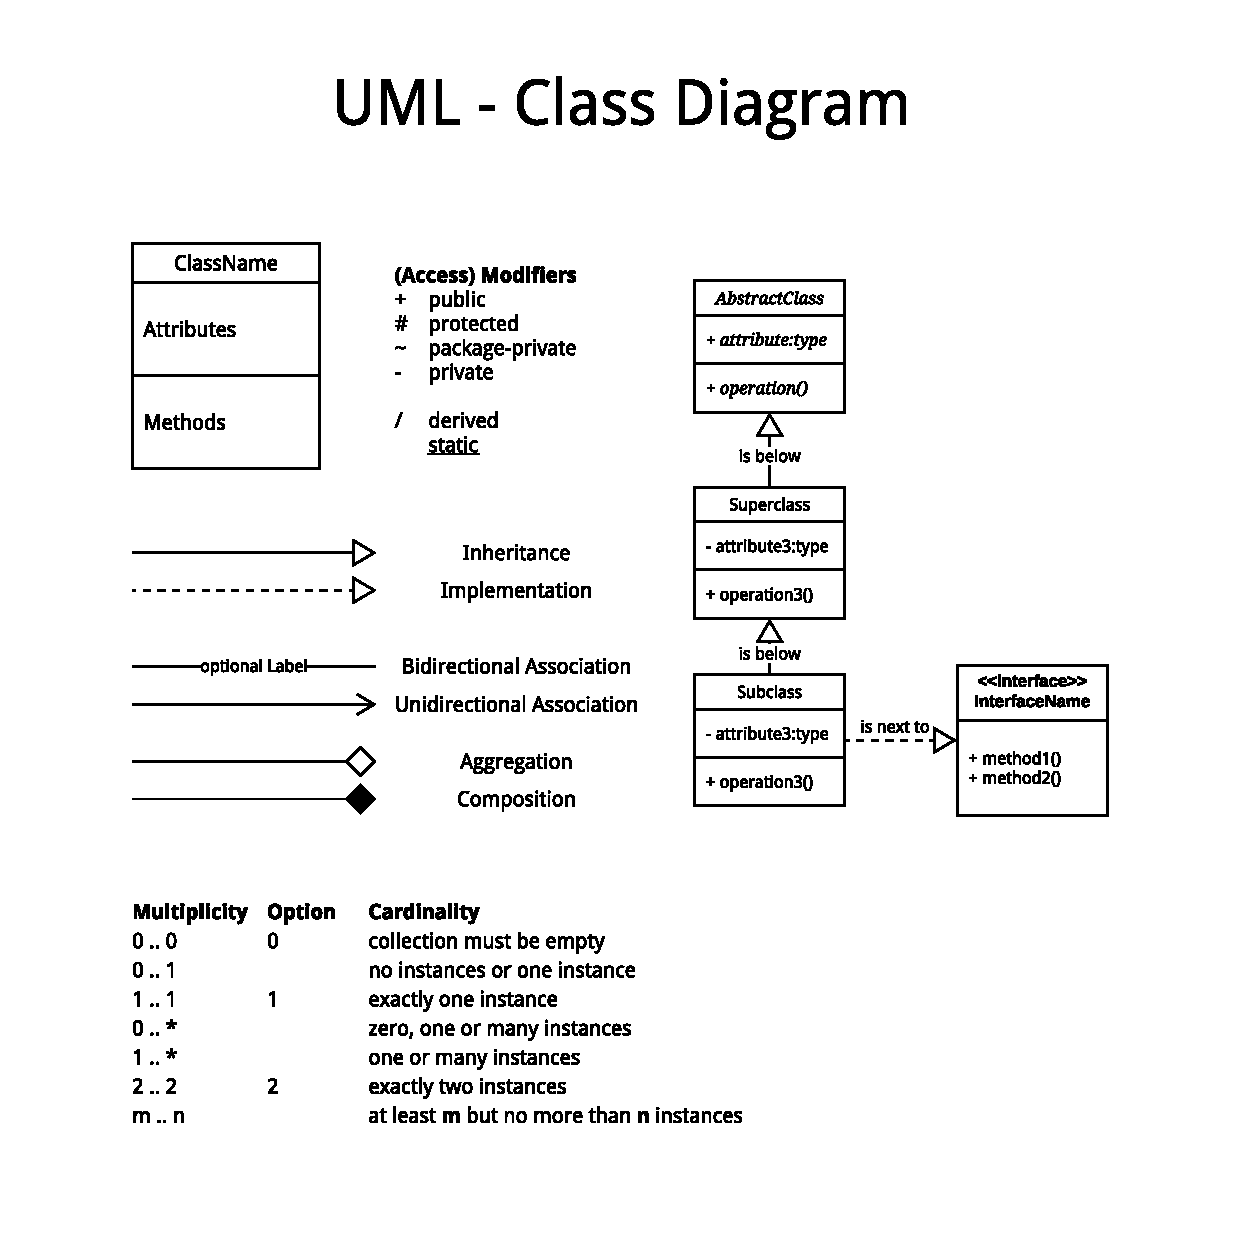
\includegraphics[width=\linewidth]{fig/UML_Classdiagram.pdf}
        \caption{Das Klassendiagramm}
        \label{fig:classdiagram}
      \end{figure}
      \newpage

\end{document}
